% !TEX root = twe2.tex

\section{Diskussion}
\label{sec:Disukussion}
\textcite[33-36]{weggler2050leguminosen} hat Möglichkeiten zur Steigerung der \ac{NEL} Erträge im Grünland aufgezeigt, allerdings ist zu beachten, dass aktuelle Verfahren der Futterkonxerierung zu hohen Verlusten führen, siehe \cref{subsec:Lit:Ernte}. \todo{ausformulieren}
Mit zukünftigen Ernte- und Konservierungsverfahren werden Landwirte hoffentlich Möglichkeiten haben die Verluste zu reduzieren.

\subsection{Literaturkritik}
\label{sub:kritik}

\begin{figure}
	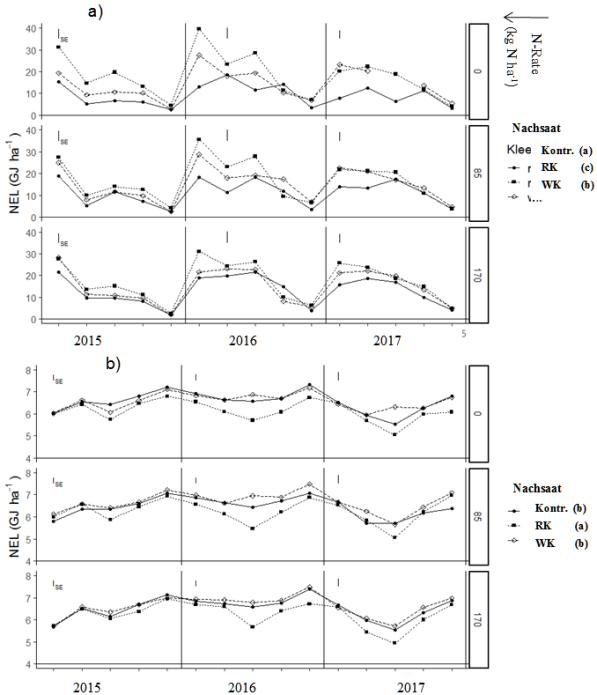
\includegraphics[scale=0.75]{images/wegglerAbb1}
	\caption[(a) \acs{NEL} Ertrag und (b) \acs{NEL} Konzentration in Abhängigkeit von der N-Düngung und Leguminosen Nachsaat über 3 Jahre]{(a) \ac{NEL} Ertrag und (b) \ac{NEL} Konzentration in Abhängigkeit von der N-Düngung und Leguminosen Nachsaat über 3 Jahre \parencite[35]{weggler2050leguminosen}}
	\label{fig:wegglerAbb1}
\end{figure}

In dem Arikel \parencite[33-36]{weggler2050leguminosen}\todo{Seitenangabe notwendig wenn die komplette Arbeit referenziert wird?} sind einige kleinere handwerkliche Fehler enthalten.
In \textcite[35]{weggler2050leguminosen} ist die Legende sowie Achsbeschriftung, siehe \cref{fig:wegglerAbb1} nicht korrekt umgesetzt.
\todo{Numerierung ok? Verwendung Abk ok?, Breite ok? Müssen Abb. linksbündig sein?}
So wird zum Beispiel der \ac{NEL} Gehalt mit GJ ha\textsuperscript{-1} beschrfitet, statt MJ kg\textsuperscript{-1} in \ac{TM}.

Desweiteren wird die Abkürzung \ac{NEL} in der Einleitung nicht als \acl{NEL} eingeführt sondern als \textit{nutzbare Energie Laktation}.\todo{kursiv okay zum makieren von Fehlern?}
Im Kapitel Material und Methoden wird \ac{NEL} als \textit{Netto Energie Lactaion} bezeichnet.
In Abbildungsunterschriften wird widerholt \textit{nutzbare Energie Laktation} verwendet.
Normalerweise wird im landwirtschaftlichen die Abkürzung \acs{NEL} für \acl{NEL} benutzt.
Desweiteren ist \ac{NEL} eine wichtige Kenngröße in der Grundfuttermittelproduktion der Milchviehhaltung und somit der Grünlandwirtschaft.
Es findet sich kein Hinweis auf eine Meßmethode welche die \textit{nutzbare Energie Laktation} bestimmt.
Daher liegt es nahe einen Fehler in der Bezeichnung zu vermuten.

Die Darstellung der \cref{fig:wegglerAbb1} ist nicht ideal.
Die verschiedenen Messpunkte beziehen sich auf die einzelnen Aufwüchse, diese per Linie miteinander zu verbinden hilft zwar beim erkennen welcher Punkt zu welcher Datenreihe gehört.
Es gitb aber keine Datenpunkte welche zwischen den einzelnen Aufwüchsen liegt, welche man eventuell interpolieren könnte.
Wen die x-Achse die N-Düngung angeben würde und die verschiedenen Schnitte in mehrere Diagramme aufgeteil worden wären, wobei bei jedem Schnitt jeweils der Durchschnitt der 3 Jahre genommen wird, wäre die Darstellung leichter verständlich.


\subsection{Leguminosen als Proteinlieferant}
\label{sub:leguminosen}
Wie in \ref{subsec:Protein} gezeigt, können Leguminosen den \ac{XP} Ertrag vom Grünland erhöhen.
Der Versuch von \textcite[33-36]{weggler2050leguminosen} wurde allerdings nur bis zu einer Düngung von 170kg N ha\textsuperscript{-1}a\textsuperscript{-1} gesteigert.
Daher ist es schwierig, einen Vergleich zwischen einer, in Norddeutschland üblichen,\todo{Zitat einfügen} N-Düngung\todo{N in Abkürzungsliste einfügen?} von über 200kg N ha\textsuperscript{-1} sowie einer minimierten N-Düngung mit Leguminosen zu ziehen.
Eine Nachsaat mit Rotklee hatte häufig einen leicht negativen Einfluss auf den \ac{XP} Gehalt des Aufwuchs, während eine Weißlkleenachsaat tendenziell eine leichte Steigerung der \ac{XP} Gehalte zur Folge hatte.
Generell sind deutliche Steigerungen des \ac{NEL} Ertrages möglich, insbesondere bei (sehr) geringer N-Düngung, wobei insbesondere der Rotklee (siehe \ref{subsec:TM}) die \ac{TM} Erträge deutlich steigert.

Da der Rotklee zu einer signifikanten Verringerung der \ac{NEL} Konzentration des Aufwuches geführt hat, ist für Milchviehbetriebe nachteilig.
Daher scheint eine Strategie mit einer Rot- Weißklee Mischung als Nachsaat für die meisten Betriebe (zumindestens kurzfristig) sinnvoll zu sein.
Bei Betrieben, welche eine etwas geringere Viehbesatzdichte haben, kann eine Weißkleenachsaat sinnvoller sein.
In weiteren Forschungen können die betriebswirtschaftlichen Einflüsse auf die Betriebe ausgearbeitet werden um den milchviehhaltenden Betrieben eine wirtschaftliche Empfehlung geben zu können.

\subsubsection{Nährstoffkreislauf}
\label{subsub:nährstoffkreislauf}

In der Milchkuhhaltung besteht ein Nährstoffkreislauf.
Über den Verkauf von Milch verlassen Nährstoffe, insbesondere N in Form des Milcheiweißes, den Betrieb.
Falls der Betrieb den Wirtschaftsdünger abgibt, bzw. abgeben muss, verlassen darüber weitere Nährstoffe den Betrieb, unter anderem N.
Nährstoffeinträge sind insbesondere über den Zukauf von Kraftfutter sowie, in eher geringen Mengen, der Einsatz von mineralischen Düngemitteln.
Der Einsatz von Kraftfuttern ist für eine Milchkuh zur Steigerung der Milchleistung sehr sinnvoll.
Eine Redufzierung des Kraftuffters ist, in den meisten Fällen, unwirtschaftlich.

Bei einer Reduzierung der N-Düngung auf den betriebseigenen Grünlandflächen ist, in den meisten Fällen, nicht mehr genügend Fläche vorhanden, um die eigenen Wirtschaftsdünger innerhalb des Betriebes zu verwerten.
Aufgrund der hohen Transportkosten ist eine Vewertung im nahem Umkreis anzustreben.
Insbesondere in Regionen mit einer hohen Besatzdichte an Milchkühen entsteht somit ein Überschuss an Wirtschaftsdüngern welcher exportiert werden muss.
Dies ist für die dort angesiedelten Betriebe eine große wirtschaftliche Herausforderung.
Nicht nur aufgrund der Transportkosten, welche in der Regel der abgebende Betrieb tragen muss, sondern auch, weil die anderen abgegeben Nährstoffe wieder zugekauft werden müssen.

\subsubsection{Leguminosen als alternative zu Kraftfutter}
\label{subsub:alternative}
Bei einem Einsatz von Leguminosen in der Grundfuttergewinnung ist eine Steigerung der \ac{NEL}-Eträge möglich.
Eine Reduzierung der Kraftfuttergabe ist, zumindestens für die meisten Betriebe, nicht wirtschaftlich.
Über das Kraftfutter wird kein Raufutter substituiert, daher ist der Einsatz von Kraftuffter unabhängig von der Qualität des Raufutters zu bewerten.

Falls Kraftfutter deutlich teuerer werden sollte, kann es sein, dass der Einsatz nicht mehr wirtschaftlich sinnvoll ist.
Die \ac{EU} könnte z.B. Importzölle auf Soja erheben, generell den Kraftfuttereinsatz einschränken oder ähnliche Einschränkungen beschließen.
Da insbesondere Soja aus Südamerika gesellschaftlich in der Kritik steht, kann es passieren, dass die \ac{EU} sich zum handeln gezwungen sieht.

Für den Fall dass der Eintrag von N über das Kraftfutter in den Nährstoffkreislauf deutlich reduziert wird, ändern sich die Vorraussetzungen.
Da der Verlust über den Verkauf von Milch bestehen bleibt, müssen neue Quellen erschlossen werden.
Eine Möglichkeit ist der Einsatz von mineralischen N-Düngemitteln, eine andere Möglichkeit wäre der Einsatz von Leguminosen.
In diesem Fall, je nach Entwicklung der Preise und bessierend auf den Ergebnissen von \textcite[33-36]{weggler2050leguminosen}, könnte eine Leguminosennachsaat kostengünstgier sein.


\subsection{Effizienz der Konservierung}
\label{sub:konservierung}
\ac{NEL} Verluste während der Ernte, Konservierung oder Lagerung sind besonders kritisch zu betrachten.
Nachdem der Landwirt aufwändig hochwertiges Futter erzeugt hat, verliert dieses etwa 20\% des \ac{NEL} Ertrags.
Diese Verluste sind aus betriebswirtschaftlicher Sicht langfristig nicht zu rechtfertigen.
Die Reduzierung dieser Verluste wird immer wichtiger, da vermutlich größere Anteile der \ac{NEL} über das Grundfutter abgedeckt werden muss.
Eine Verbesserung der Ernteverfahren bzw. Konservierungsmethoden ist daher dringend geboten.
Es bleibt somit zu hoffen dass die Forschung neue wirtschaftliche Verfahren entwickelt welche eine wirtschaftliche Nutzung des kompletten \ac{NEL} Ertrags von landwirtschaftlichen Flächen erlaubt.

\subsection{Fazit}
\label{subsec:fazit}
Leguminosen sind eine sinnvolle Variante um die \ac{NEL} Erträge des Grünlandes zu steigern.
Neben der Steigerung der Erträge wäre eine effizientere Verwertung dieser wünschenswert.
